\documentclass{article}
\usepackage{tikz}
\usetikzlibrary{shapes.geometric,calc,angles,positioning,intersections,quotes,decorations,babel,patterns,fit}
\usepackage{tkz-euclide}
\usetkzobj{all}
\begin{document}
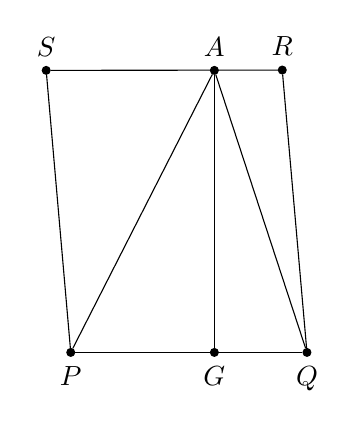
\begin{tikzpicture}
[scale =0.6,>=stealth,point/.style = {draw, circle, fill = black, inner sep = 1pt},]
\node (S) at (-0.52,5.97)[point,label=above :$S$] {};
\node (P) at (0,0)[point,label=below :$P$] {};
\node (A) at (3.04,5.97)[point,label=above :$A$] {};
\node (R) at (4.477,5.977)[point,label=above :$R$] {};
\node (G) at (3.04,0)[point,label=below:$G$] {};
\node (Q) at (5,0)[point,label=below :$Q$] {};
\draw (S)--(P);
\draw (P)--(Q);
\draw (Q)--(R);
\draw (R)--(S);
\draw (A)--(P);
\draw (A)--(Q);
\draw (A)--(G);
\end{tikzpicture}
\end{document}